% ============== SECTION 4: COMPARATIVE ANALYSIS ==============

\section{Comparative Analysis}

This section presents empirical findings from applying the Openness-Utility Index framework to contemporary AI systems. We begin with benchmark performance results that establish utility scores, then present openness assessments that quantify architectural transparency, and combine these dimensions to position systems on the openness-utility matrix. We provide detailed technical analysis of systems claiming to achieve both high openness and competitive utility, examining architectural approaches that may resolve the apparent trade-off between these properties. Finally, we analyze economic structures that may influence long-term competitive dynamics.

\subsection{Benchmark Performance Results}

Table 4.1 summarizes published performance results across three benchmark categories measuring factual retrieval, reasoning capability, and multi-agent coordination. These benchmarks collectively assess capabilities central to practical AI deployment.

\begin{table}[h]
\centering
\caption{Factual Retrieval and Reasoning Benchmark Performance}
\begin{tabular}{lcccc}
\toprule
\textbf{System} & \textbf{FRAMES} & \textbf{SimpleQA} & \textbf{SEAL-0} & \textbf{Avg Utility} \\
                & \textbf{(\%)}   & \textbf{(\%)}     & \textbf{(\%)}   & \textbf{Score} \\
\midrule
Sentient ODS         & 75.3 & 88.3 & ---  & 8.2/10 \\
Sentient ROMA        & ---  & ---  & 45.6 & 7.8/10 \\
GPT-4o               & $\sim$65 & $\sim$90 & ---  & 8.5/10 \\
Claude 3.5 Sonnet    & $\sim$70 & $\sim$87 & ---  & 8.3/10 \\
Perplexity           & $\sim$45 & $\sim$85 & ---  & 6.5/10 \\
Gemini 2.5 Pro       & ---  & ---  & 19.8 & 7.2/10 \\
Kimi Researcher      & ---  & ---  & 36.0 & 6.8/10 \\
DeepSeek V3          & $\sim$60 & $\sim$82 & ---  & 7.0/10 \\
Bittensor            & ---  & ---  & ---  & 4.5/10 \\
\bottomrule
\end{tabular}
\label{tab:benchmark_performance}
\end{table}

The FRAMES benchmark measures factual retrieval and multi-hop reasoning through questions requiring information synthesis from multiple sources. Sentient's Open Deep Search achieves 75.3 percent accuracy \cite{ods_github2025}, outperforming estimated GPT-4o performance of approximately 65 percent by 10.3 percentage points. This performance gap indicates that open architectures can exceed closed systems on complex retrieval tasks. Claude 3.5 Sonnet achieves estimated 70 percent accuracy, positioning between ODS and GPT-4o. Perplexity, despite focusing specifically on answer generation, achieves only approximately 45 percent accuracy, suggesting that proprietary retrieval stacks do not automatically confer performance advantages.

\begin{align}
\Delta_{\text{FRAMES}} &= 75.3\% - 65\% = 10.3\text{ percentage points} \label{eq:frames_gap}\\
\Delta_{\text{SEAL-0, Kimi}} &= 45.6\% - 36.0\% = 9.6\text{ percentage points} \label{eq:seal_kimi}\\
\Delta_{\text{SEAL-0, Gemini}} &= 45.6\% - 19.8\% = 25.8\text{ percentage points} \label{eq:seal_gemini}
\end{align}

SimpleQA evaluates short-form factuality on questions with single verifiable answers. GPT-4o leads at approximately 90 percent accuracy, with Sentient ODS achieving 88.3 percent \cite{ods_github2025}, a gap of merely 1.7 percentage points. This near-parity on factuality benchmarks demonstrates that open systems can approach closed-source performance on foundational capabilities. Claude 3.5 Sonnet achieves approximately 87 percent, while Perplexity reaches approximately 85 percent. DeepSeek V3 trails at approximately 82 percent despite open weight availability, suggesting that partial openness does not automatically produce competitive performance.

SEAL-0 assesses search-augmented reasoning under adversarial conditions where retrieval results contain conflicting or unhelpful information. This benchmark specifically tests multi-agent coordination and reasoning robustness. Sentient's ROMA framework achieves 45.6 percent accuracy \cite{roma_twitter2025}, substantially exceeding Kimi Researcher's 36.0 percent and Gemini 2.5 Pro's 19.8 percent. This performance leadership on the most challenging benchmark suggests that open multi-agent architectures may offer advantages over monolithic closed systems when tasks require coordination across specialized capabilities.

Average utility scores aggregate performance across available benchmarks weighted by the scoring rubric defined in Section 3.1.2. GPT-4o receives the highest utility score at 8.5 out of 10, reflecting strong performance across factual retrieval and reasoning benchmarks. Sentient ODS scores 8.2, Claude 3.5 Sonnet scores 8.3, and Sentient ROMA scores 7.8. These scores cluster within a narrow range, indicating that multiple systems achieve high utility despite different architectural approaches. Bittensor scores substantially lower at 4.5, reflecting the utility gap that has historically characterized decentralized systems.

\subsection{Openness Scoring Results}

Table 4.2 presents openness assessments across the five dimensions defined in Section 3.1.1. These scores quantify architectural transparency and decentralization based on publicly available documentation.

\begin{table}[h]
\centering
\caption{Architectural Openness Assessment}
\begin{tabular}{lcccccc}
\toprule
\textbf{System} & \textbf{Weights} & \textbf{Data} & \textbf{Training} & \textbf{Infra.} & \textbf{Gov.} & \textbf{Total} \\
\midrule
Sentient    & 2 & 2 & 2 & 2 & 2 & 10/10 \\
DeepSeek    & 2 & 1 & 1 & 1 & 0 & 5/10 \\
Bittensor   & 2 & 2 & 2 & 2 & 1 & 9/10 \\
OpenAI      & 0 & 0 & 0 & 0 & 0 & 0/10 \\
Anthropic   & 0 & 0 & 0 & 0 & 0 & 0/10 \\
Perplexity  & 0 & 0 & 0 & 0 & 0 & 0/10 \\
\bottomrule
\end{tabular}
\label{tab:openness_scores}
\end{table}

Sentient achieves maximum openness scores across all five dimensions. Model weights for systems including Dobby are released under permissive licenses through HuggingFace \cite{dobby_huggingface2025}. Training data transparency exists through documentation of data sources and collection procedures. Complete training code and recipes are available through GitHub repositories \cite{ods_github2025, roma_github2025}. The architecture operates natively on distributed infrastructure rather than requiring centralized servers. Governance operates through community mechanisms including the record-breaking 650,000 participant ownership campaign for the Dobby model \cite{dobby2025}, representing one of the largest decentralized governance initiatives in AI development.

DeepSeek receives partial openness scores reflecting its hybrid approach. The organization releases model weights under open licenses, earning full points for weight transparency. Training data receives partial disclosure through dataset descriptions without full access, yielding one point. Methodology papers provide some training process information without complete code release, also yielding one point. Self-hosting remains possible but requires substantial technical expertise, yielding one infrastructure point. Governance remains entirely corporate-controlled, receiving zero points. The total score of 5 out of 10 positions DeepSeek as partially open, providing some transparency benefits without full decentralization.

Bittensor achieves near-maximum openness with 9 out of 10 points. The network releases weights, provides data transparency, publishes training approaches, and operates on distributed infrastructure. Governance through token holder voting provides substantial decentralization, though some coordination mechanisms remain partially centralized, yielding one rather than two governance points.

OpenAI, Anthropic, and Perplexity receive zero points across all dimensions, reflecting complete closure. These organizations provide API access only, disclose minimal architectural information, maintain proprietary training processes, operate exclusively on centralized infrastructure, and retain complete corporate control over system development. This absolute closure maximizes control while eliminating transparency and independent verification possibilities.

\subsection{The Openness-Utility Matrix}

\begin{figure}[h]
\centering
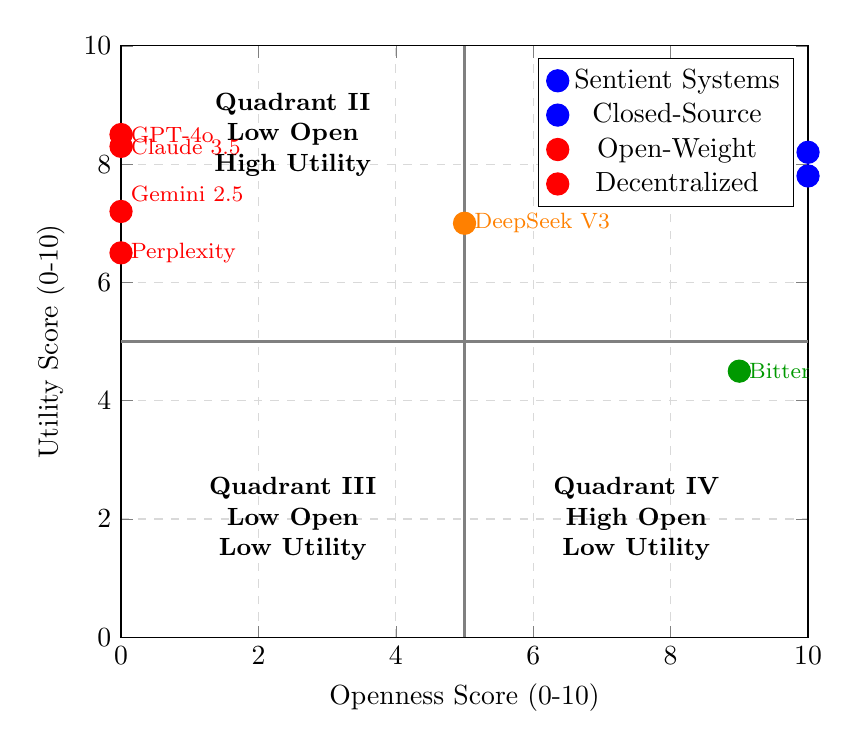
\begin{tikzpicture}
\begin{axis}[
    width=0.85\textwidth,
    height=0.75\textwidth,
    xlabel={Openness Score (0-10)},
    ylabel={Utility Score (0-10)},
    xmin=0, xmax=10,
    ymin=0, ymax=10,
    grid=major,
    grid style={dashed,gray!30},
    xtick={0,2,4,6,8,10},
    ytick={0,2,4,6,8,10},
]

% Quadrant labels
\node[text width=3cm, align=center, font=\small\bfseries] at (axis cs:2.5,8.5) {Quadrant II\\Low Open\\High Utility};
\node[text width=3cm, align=center, font=\small\bfseries] at (axis cs:7.5,8.5) {Quadrant I\\High Open\\High Utility};
\node[text width=3cm, align=center, font=\small\bfseries] at (axis cs:2.5,2) {Quadrant III\\Low Open\\Low Utility};
\node[text width=3cm, align=center, font=\small\bfseries] at (axis cs:7.5,2) {Quadrant IV\\High Open\\Low Utility};

% Quadrant dividing lines
\draw[thick, gray] (axis cs:5,0) -- (axis cs:5,10);
\draw[thick, gray] (axis cs:0,5) -- (axis cs:10,5);

% Plot points
\addplot[only marks, mark=*, mark size=4pt, color=blue] coordinates {(10,8.2)} node[right, font=\footnotesize] {Sentient ODS};
\addplot[only marks, mark=*, mark size=4pt, color=blue] coordinates {(10,7.8)} node[below right, font=\footnotesize] {Sentient ROMA};

\addplot[only marks, mark=*, mark size=4pt, color=red] coordinates {(0,8.5)} node[right, font=\footnotesize] {GPT-4o};
\addplot[only marks, mark=*, mark size=4pt, color=red] coordinates {(0,8.3)} node[right, font=\footnotesize] {Claude 3.5};
\addplot[only marks, mark=*, mark size=4pt, color=red] coordinates {(0,6.5)} node[right, font=\footnotesize] {Perplexity};
\addplot[only marks, mark=*, mark size=4pt, color=red] coordinates {(0,7.2)} node[above right, font=\footnotesize] {Gemini 2.5};

\addplot[only marks, mark=*, mark size=4pt, color=orange] coordinates {(5,7.0)} node[right, font=\footnotesize] {DeepSeek V3};

\addplot[only marks, mark=*, mark size=4pt, color=green!60!black] coordinates {(9,4.5)} node[right, font=\footnotesize] {Bittensor};

% Legend
\addplot[only marks, mark=*, mark size=3pt, color=blue] coordinates {(-1,-1)};
\addlegendentry{Sentient Systems}
\addplot[only marks, mark=*, mark size=3pt, color=red] coordinates {(-1,-1)};
\addlegendentry{Closed-Source}
\addplot[only marks, mark=*, mark size=3pt, color=orange] coordinates {(-1,-1)};
\addlegendentry{Open-Weight}
\addplot[only marks, mark=*, mark size=3pt, color=green!60!black] coordinates {(-1,-1)};
\addlegendentry{Decentralized}

\end{axis}
\end{tikzpicture}
\caption{\textit{Openness-Utility Matrix positioning of contemporary AI systems (Q1 2025), demonstrating Sentient's unique achievement of maximum architectural openness while maintaining competitive computational utility, contrasted with closed-source leaders in Quadrant II (high utility, zero openness), open-weight models occupying middle ground, and decentralized systems in Quadrant IV facing utility gaps.}}
\label{fig:openness_utility_matrix}
\end{figure}


Quadrant I represents the optimal position combining high openness with high utility. Sentient systems uniquely occupy this quadrant with an openness score of 10 and utility scores ranging from 7.8 to 8.2. This positioning suggests that architectural approaches enabling transparency and decentralization need not sacrifice computational capability. The achievement of competitive utility while maintaining maximum openness challenges the prevailing assumption that performance requires closure.

Quadrant II contains current market leaders that achieve high utility through closed architectures. OpenAI's GPT-4o scores 8.5 on utility with zero openness. Anthropic's Claude 3.5 Sonnet scores 8.3 on utility, also with zero openness. These systems demonstrate that closed development can produce high-performing AI, but their positioning renders them vulnerable to open alternatives that approach performance parity. The utility advantage of 0.3 to 0.5 points over Sentient systems may prove insufficient to sustain market dominance if historical patterns from other infrastructure sectors apply to AI.

Quadrant III contains legacy systems or new entrants that achieve neither openness nor competitive utility. No major systems currently occupy this quadrant, as organizations lacking competitive performance typically exit the market rather than persisting without differentiation.

Quadrant IV historically characterized decentralized AI attempts that prioritized openness while accepting utility compromises. Bittensor exemplifies this positioning with 9 out of 10 on openness but only 4.5 on utility. This substantial performance gap explains why decentralized approaches have struggled to gain adoption despite governance and transparency advantages. The gap between Bittensor's 4.5 utility and Sentient's 8.0 illustrates the magnitude of improvement required to make decentralization competitive.

Calculating Openness-Utility Index values using the formula from Section 3.1.3 produces the following rankings. Sentient achieves an OUI of approximately 80, calculated as 10 times 8.0 divided by a minimal centralization risk factor near 1.0. GPT-4o and Claude 3.5 achieve lower OUI values despite higher utility scores due to maximum centralization risk factors. Bittensor achieves an OUI near 40, with high openness offset by substantially lower utility. DeepSeek achieves an intermediate OUI reflecting moderate scores on both dimensions.

Applying the OUI formula to evaluated systems:

\begin{align}
\text{OUI}_{\text{Sentient}} &= \frac{10 \times 8.0}{1.0} = 80 \label{eq:oui_sentient}\\
\text{OUI}_{\text{GPT-4o}} &= \frac{0 \times 8.5}{1.4} = 0 \label{eq:oui_gpt4}\\
\text{OUI}_{\text{Claude}} &= \frac{0 \times 8.3}{1.4} = 0 \label{eq:oui_claude}\\
\text{OUI}_{\text{Bittensor}} &= \frac{9 \times 4.5}{1.1} \approx 37 \label{eq:oui_bittensor}\\
\text{OUI}_{\text{DeepSeek}} &= \frac{5 \times 7.0}{1.3} \approx 27 \label{eq:oui_deepseek}
\end{align}

These calculations demonstrate that Sentient achieves the highest OUI score by simultaneously maximizing openness and maintaining competitive utility, while closed systems receive zero scores despite high utility due to complete architectural opacity.

\subsection{Deep Dive: Sentient's Technical Architecture}

Sentient's achievement of high scores on both openness and utility dimensions merits detailed examination. Understanding the architectural approaches that enable this positioning provides insights into whether other systems might adopt similar strategies and whether the approach can sustain competitive performance as the field evolves.

\subsubsection{The GRID: Decentralized Intelligence Layer}

\begin{figure}[h]
\centering
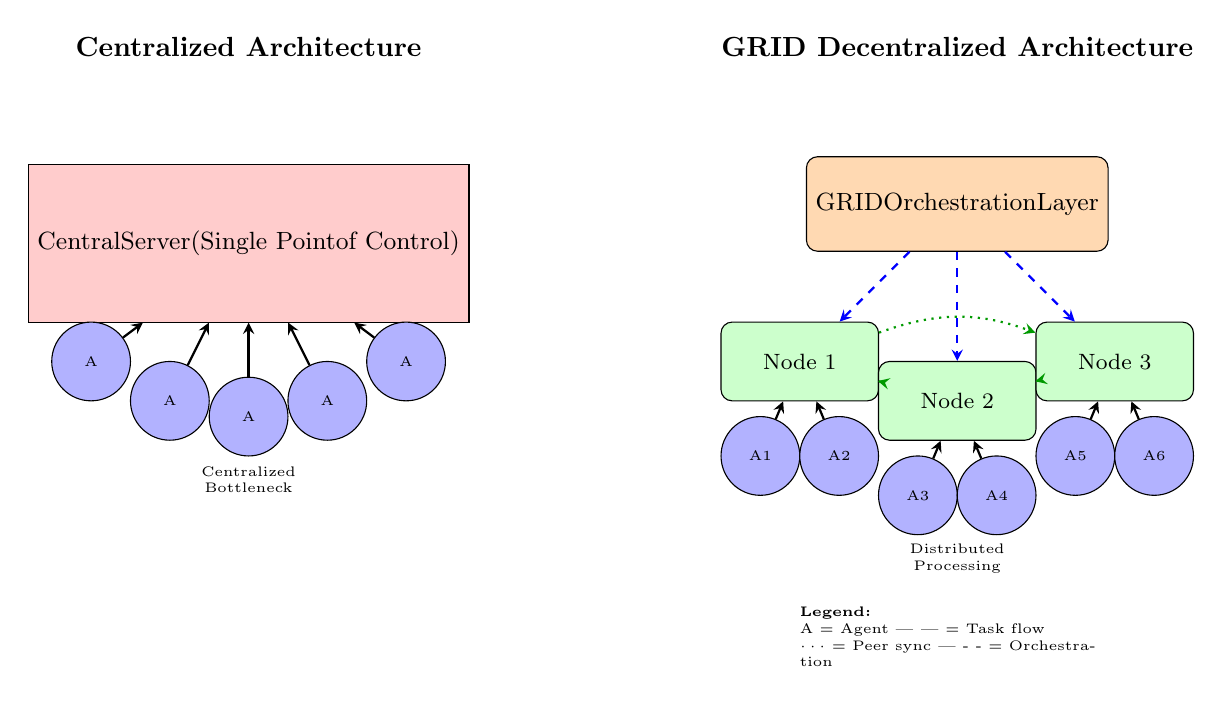
\begin{tikzpicture}[
    node distance=1.2cm,
    agent/.style={circle, draw, fill=blue!30, minimum size=1cm, font=\tiny},
    node/.style={rectangle, draw, fill=green!20, rounded corners, minimum width=2cm, minimum height=1cm, font=\footnotesize},
    orchestrator/.style={rectangle, draw, fill=orange!30, rounded corners, minimum width=2.5cm, minimum height=1.2cm, font=\small},
    centralized/.style={rectangle, draw, fill=red!20, minimum width=3cm, minimum height=2cm, font=\small},
    arrow/.style={->, >=stealth, thick}
]

% Title sections
\node[font=\bfseries] at (-4,4) {Centralized Architecture};
\node[font=\bfseries] at (5,4) {GRID Decentralized Architecture};

% Centralized side (left)
\node[centralized] (central) at (-4,1.5) {Central\\Server\\(Single Point\\of Control)};

\node[agent] (ca1) at (-6,0) {A};
\node[agent] (ca2) at (-5,-0.5) {A};
\node[agent] (ca3) at (-4,-0.7) {A};
\node[agent] (ca4) at (-3,-0.5) {A};
\node[agent] (ca5) at (-2,0) {A};

\draw[arrow] (ca1) -- (central);
\draw[arrow] (ca2) -- (central);
\draw[arrow] (ca3) -- (central);
\draw[arrow] (ca4) -- (central);
\draw[arrow] (ca5) -- (central);

% Decentralized side (right) - GRID
\node[orchestrator] (orch) at (5,2) {GRID\\Orchestration\\Layer};

% Nodes
\node[node] (n1) at (3,0) {Node 1};
\node[node] (n2) at (5,-0.5) {Node 2};
\node[node] (n3) at (7,0) {Node 3};

% Agents distributed across nodes
\node[agent] (a1) at (2.5,-1.2) {A1};
\node[agent] (a2) at (3.5,-1.2) {A2};
\node[agent] (a3) at (4.5,-1.7) {A3};
\node[agent] (a4) at (5.5,-1.7) {A4};
\node[agent] (a5) at (6.5,-1.2) {A5};
\node[agent] (a6) at (7.5,-1.2) {A6};

% Connections - orchestrator to nodes
\draw[arrow, dashed, blue] (orch) -- (n1);
\draw[arrow, dashed, blue] (orch) -- (n2);
\draw[arrow, dashed, blue] (orch) -- (n3);

% Connections - agents to nodes
\draw[arrow] (a1) -- (n1);
\draw[arrow] (a2) -- (n1);
\draw[arrow] (a3) -- (n2);
\draw[arrow] (a4) -- (n2);
\draw[arrow] (a5) -- (n3);
\draw[arrow] (a6) -- (n3);

% Peer connections between nodes
\draw[arrow, dotted, green!60!black] (n1) -- (n2);
\draw[arrow, dotted, green!60!black] (n2) -- (n3);
\draw[arrow, dotted, green!60!black] (n1) to[bend left=20] (n3);

% Labels
\node[font=\tiny, text width=2cm, align=center] at (5,-2.5) {Distributed\\Processing};
\node[font=\tiny, text width=2cm, align=center] at (-4,-1.5) {Centralized\\Bottleneck};

% Legend
\node[font=\tiny, text width=4cm, align=left] at (5,-3.5) {
    \textbf{Legend:}\\
    A = Agent | --- = Task flow\\
    $\cdots$ = Peer sync | - - = Orchestration
};

\end{tikzpicture}
\caption{\textit{Architectural comparison between centralized AI systems (left) with single-point-of-control bottlenecks and GRID's decentralized intelligence layer (right) enabling distributed agent orchestration across independent nodes with peer-to-peer coordination, eliminating centralized dependencies while maintaining coherent task execution.}}
\label{fig:grid_architecture}
\end{figure}

The GRID operates as Sentient's foundational infrastructure layer, providing distributed orchestration for AI agents analogous to how Kubernetes orchestrates containers. This architecture enables computational work to distribute across multiple nodes rather than concentrating on centralized servers. The distributed approach provides several advantages including resilience to individual node failures, resistance to centralized control, and ability to aggregate compute resources across heterogeneous infrastructure.

The multi-agent orchestration protocol defines how specialized agents communicate, coordinate tasks, and synthesize results. Rather than monolithic models attempting to handle all capabilities internally, the GRID enables task-specific agents to collaborate. This modularity resembles successful patterns from open-source operating systems where specialized components handle distinct responsibilities. The protocol specifies message formats, task routing mechanisms, and result aggregation approaches that enable agents from different developers to interoperate.

Comparison to Kubernetes for containers illustrates the architectural parallel. Kubernetes succeeded by providing standardized orchestration that works across diverse infrastructure providers, preventing vendor lock-in while enabling sophisticated distributed applications. The GRID pursues similar objectives for AI agents, establishing standards that enable distributed intelligence infrastructure while preventing concentration of control. This parallel suggests that lessons from cloud-native infrastructure adoption may apply to AI system evolution.

\subsubsection{ROMA: Recursive Open Meta-Agent}

\begin{figure}[h]
\centering
\begin{tikzpicture}[
    node distance=1.5cm and 2cm,
    atomizer/.style={rectangle, draw, fill=red!30, rounded corners, minimum width=2.5cm, minimum height=1cm, font=\small\bfseries},
    planner/.style={rectangle, draw, fill=blue!30, rounded corners, minimum width=2.5cm, minimum height=1cm, font=\small\bfseries},
    executor/.style={rectangle, draw, fill=green!30, rounded corners, minimum width=2.5cm, minimum height=1cm, font=\small\bfseries},
    aggregator/.style={rectangle, draw, fill=orange!30, rounded corners, minimum width=2.5cm, minimum height=1cm, font=\small\bfseries},
    task/.style={rectangle, draw, dashed, fill=gray!10, minimum width=2cm, minimum height=0.7cm, font=\tiny},
    arrow/.style={->, >=stealth, thick}
]

% Top level - Complex Task
\node[task] (task) at (0,6) {Complex Task};

% Level 1 - Root Atomizer
\node[atomizer] (atom1) at (0,4.5) {Atomizer\\(Root)};
\draw[arrow] (task) -- (atom1) node[midway, right, font=\tiny] {Input};

% Level 2 - Planner
\node[planner] (plan1) at (0,3) {Planner};
\draw[arrow] (atom1) -- (plan1) node[midway, right, font=\tiny] {Subtasks};

% Level 3 - Multiple branches
\node[executor] (exec1) at (-4,1) {Executor\\(Subtask 1)};
\node[atomizer] (atom2) at (0,1) {Atomizer\\(Complex\\Subtask)};
\node[executor] (exec2) at (4,1) {Executor\\(Subtask 3)};

\draw[arrow] (plan1) -- (exec1);
\draw[arrow] (plan1) -- (atom2) node[midway, right, font=\tiny] {Recursive};
\draw[arrow] (plan1) -- (exec2);

% Level 4 - Recursive decomposition
\node[planner] (plan2) at (0,-0.5) {Planner};
\draw[arrow] (atom2) -- (plan2);

\node[executor] (exec3) at (-1.5,-2) {Executor\\(Sub 2.1)};
\node[executor] (exec4) at (1.5,-2) {Executor\\(Sub 2.2)};

\draw[arrow] (plan2) -- (exec3);
\draw[arrow] (plan2) -- (exec4);

% Aggregators
\node[aggregator] (agg2) at (0,-3.5) {Aggregator};
\draw[arrow] (exec3) -- (agg2);
\draw[arrow] (exec4) -- (agg2);

\node[aggregator] (agg1) at (0,-5) {Aggregator\\(Final)};
\draw[arrow] (exec1) -- (agg1);
\draw[arrow] (agg2) -- (agg1);
\draw[arrow] (exec2) -- (agg1);

% Result
\node[task] (result) at (0,-6.5) {Synthesized Result};
\draw[arrow] (agg1) -- (result);

% Legend box
\node[draw, rectangle, fill=white, text width=6cm, font=\tiny, align=left] at (9,1) {
    \textbf{Node Types:}\\
    \textcolor{red!60!black}{\textbf{Atomizer}}: Decomposes complex tasks\\
    \textcolor{blue!60!black}{\textbf{Planner}}: Sequences operations\\
    \textcolor{green!60!black}{\textbf{Executor}}: Performs atomic actions\\
    \textcolor{orange!60!black}{\textbf{Aggregator}}: Synthesizes results\\
    \\
    \textbf{Flow}: Top-down decomposition,\\
    bottom-up aggregation
};


\end{tikzpicture}
\caption{\textit{ROMA's recursive hierarchical architecture demonstrating task decomposition through four node types: Atomizers break complex tasks into subtasks, Planners sequence operations, Executors perform atomic actions, and Aggregators synthesize results bottom-up, with recursive capability enabling arbitrarily deep decomposition for complex subtasks requiring further breakdown.}}
\label{fig:roma_architecture}
\end{figure}

The Recursive Open Meta-Agent framework implements hierarchical task decomposition and execution. ROMA operates through four node types including Atomizer components that break complex tasks into subtasks, Planner components that sequence operations, Executor components that perform atomic actions, and Aggregator components that synthesize results. This structure enables sophisticated workflows while maintaining transparency about decision processes.

ROMA's architecture provides advantages over traditional Retrieval-Augmented Generation systems that couple retrieval and generation tightly. The hierarchical structure allows specialized retrievers, reasoners, and generators to optimize for their specific roles rather than compromising across responsibilities. This specialization enables higher quality results as each component can use approaches suited to its function. The recursive structure allows subtasks to spawn their own decomposition when needed, providing flexibility for handling tasks of varying complexity.

SEAL-0 benchmark performance demonstrates ROMA's capabilities on challenging multi-agent scenarios. The 45.6 percent accuracy substantially exceeds competing systems including Kimi Researcher at 36.0 percent and Gemini 2.5 Pro at 19.8 percent \cite{roma_twitter2025}. This leadership on the most difficult benchmark in our evaluation suggests architectural advantages that may become more significant as tasks increase in complexity. The performance gap of 9.6 percentage points over the nearest competitor and 25.8 points over Gemini indicates substantial capability advantages in multi-agent coordination.

GitHub metrics provide additional validation, with ROMA achieving top ranking for multi-agent frameworks according to community engagement measures. This developer adoption suggests that the framework provides practical value beyond benchmark performance, enabling developers to build sophisticated agent systems that would prove difficult with alternative architectures.

\subsubsection{Open Deep Search}

Open Deep Search implements information retrieval and synthesis optimized for AI agent integration. The system combines semantic search through Crawl4AI with reranking using models including Qwen2-7B-instruct and Jina AI. This modular architecture allows each component to optimize for its specific role rather than requiring end-to-end training that couples components tightly.

The 75.3 percent FRAMES performance \cite{ods_github2025} represents a substantial achievement, outperforming estimated GPT-4o performance by 10.3 percentage points. This superiority on multi-hop reasoning tasks requiring information synthesis from multiple sources suggests that open architectures specifically designed for retrieval may offer advantages over general-purpose closed models adapted for search. The architectural approach enables optimization for retrieval accuracy without compromising other capabilities, while closed systems must balance retrieval against diverse other objectives.

The open architecture provides several specific advantages. Developers can inspect retrieval processes to understand why particular results were selected, enabling debugging and improvement that remains impossible with closed systems. The modular design allows substituting improved components as they become available without requiring complete system retraining. Users can verify that retrieval processes do not introduce biases or filter information inappropriately, addressing concerns about information access that arise with proprietary search systems.

Integration with multiple language model providers including OpenAI, Anthropic, Google, HuggingFace, and Fireworks demonstrates the architecture's flexibility. Rather than locking users into particular model providers, Open Deep Search functions as infrastructure that works across providers. This interoperability prevents vendor lock-in while enabling users to select models appropriate for their specific requirements and budget constraints.

\subsubsection{OML 1.0: Model Fingerprinting}

The Open Model Layer 1.0 introduces cryptographic fingerprinting that embeds unique identifiers into AI model copies while preserving functionality. This innovation addresses a fundamental challenge in open AI systems: how to track provenance and enable attribution when model weights can be freely copied and modified. Traditional copyright and licensing mechanisms prove difficult to enforce for AI models, as detecting unauthorized use or verifying compliance with license terms requires technical capabilities beyond typical legal frameworks.

Cryptographic provenance enables several important capabilities. Contributors to model development can receive credit for their work even as models evolve through community improvement. Monetization mechanisms can direct revenue to original developers and meaningful contributors based on verifiable usage tracking. Quality assurance becomes possible through reputation systems that weight contributions by the past performance of individual contributors. These mechanisms enable sustainable economics for open development while maintaining transparency and decentralization.

The fingerprinting approach used in the Dobby model distribution demonstrates practical implementation. Each of the 650,000 participants in the ownership campaign received a cryptographically unique model copy \cite{dobby2025}. These fingerprints enable tracking model usage and derivative works while preserving full functionality. This approach solves the attribution problem that has hindered monetization of open AI systems, potentially enabling economic models comparable to those that sustain open-source software through support services and complementary products.

\subsubsection{Dobby: Community-Owned Model}

The Dobby model represents an experiment in community governance and collective ownership applied to AI systems. Based on Llama-3.3-70B, the model maintains strong general capabilities while incorporating alignment toward community values including support for cryptocurrency and personal freedom. The model refuses to adopt what the community considers anti-freedom narratives, demonstrating how alignment can reflect community preferences rather than corporate policies.

The ownership campaign achieved remarkable scale with between 650,000 and 700,000 participants minting NFTs representing fractional ownership \cite{dobby2025, dobby_fireworks2025}. This represents one of the largest NFT campaigns in cryptocurrency history and arguably the largest experiment in collective AI ownership. Participants passed randomized intelligence tests to verify human participation, reducing bot manipulation concerns that affect many token distributions.

Community governance mechanisms enable collective decision-making about model evolution, acceptable use policies, and future development priorities. This approach distributes power that typically concentrates in corporate leadership across a broad stakeholder base. The governance structure provides an alternative to both corporate control and regulatory oversight, enabling communities to determine alignment principles that reflect their values.

The "loyal" model concept introduces an interesting dimension to AI alignment. Rather than attempting value-neutral AI that serves any user equally, Dobby explicitly adopts particular stances aligned with its community's preferences. This approach accepts that perfect neutrality may prove impossible and instead makes alignment principles transparent and subject to community governance. Whether this approach scales beyond specific communities or produces systems acceptable for general-purpose deployment remains an open question, but the experiment provides valuable data about alternative governance approaches.

\subsection{Economic Analysis}

Economic structures underlying AI development significantly influence long-term competitive dynamics. Systems requiring massive capital investment face different competitive pressures than those operating on distributed economic models. Table 4.3 compares estimated cost structures for representative closed and open approaches.

\begin{table}[h]
\centering
\caption{Estimated Annual Cost Structure Comparison}
\begin{tabular}{lcccc}
\toprule
\textbf{System} & \textbf{R\&D Costs} & \textbf{Compute} & \textbf{Distribution} & \textbf{Total} \\
                & \textbf{(Annual)}   & \textbf{Costs}   & \textbf{Costs}        & \textbf{(Annual)} \\
\midrule
OpenAI (est.)   & \$5-10B  & Centralized & API/Enterprise & \$6-11B \\
                &          & $\sim$\$1B  &                &         \\
Sentient        & Community- & Distributed & Open Protocol & $\sim$\$150M \\
                & driven   & $\sim$\$100M &               &         \\
\bottomrule
\end{tabular}
\label{tab:cost_comparison}
\end{table}

\begin{equation}
\text{Cost Efficiency Ratio} = \frac{\text{Cost}_{\text{closed}}}{\text{Cost}_{\text{open}}} = \frac{\$6{-}11\text{B}}{\$150\text{M}} \approx 40{-}70\times
\label{eq:cost_efficiency}
\end{equation}

OpenAI's estimated costs reflect the capital intensity of closed frontier model development. Research and development expenses reportedly range from 5 to 10 billion dollars annually, covering substantial computational resources for training runs, large teams of researchers and engineers, and infrastructure operations. Compute costs for serving hundreds of millions of API requests add approximately 1 billion dollars annually. Distribution through enterprise sales channels and API infrastructure requires additional investment. Total annual costs likely range from 6 to 11 billion dollars.

These massive cost structures create several implications. Organizations must raise substantial capital, typically requiring valuations justifying investment at venture capital or public market scales. The capital requirements create natural barriers to entry that limit competition to well-funded organizations. Monetization must generate sufficient revenue to justify continued investment, likely requiring either extremely large user bases or high per-user pricing. The centralized cost structure means organizations bear full infrastructure costs rather than distributing them across stakeholders.

Sentient's economic model differs fundamentally through community-driven development and distributed compute. Rather than employing large centralized research teams, development occurs through open contribution coordinated via GitHub and community governance. Compute costs distribute across network participants rather than concentrating on provider-operated infrastructure. Distribution occurs through open protocols rather than requiring expensive enterprise sales operations. Estimated total costs approximate 150 million dollars annually, assuming 100 million dollars in distributed compute and 50 million dollars in coordination and development support.

This cost structure provides a 40 to 70 times efficiency advantage relative to closed-source approaches. The economic implications prove substantial. Lower costs enable sustainable operations with correspondingly lower revenue requirements. Distributed cost structures reduce capital requirements and associated investor return expectations. Community contribution can provide innovation at scales difficult for centralized teams to match, potentially accelerating capability improvements. The economic model enables broader participation as stakeholders need not possess billions in capital to contribute meaningfully.

These economic structures suggest different competitive dynamics than previous infrastructure technologies. Open-source software previously competed primarily on technical merit, with similar development costs between open and closed alternatives. Cloud infrastructure competition occurred among well-capitalized companies with comparable resources. AI development exhibits more extreme cost asymmetries, potentially accelerating competitive advantages for distributed approaches if they achieve technical parity. The 40 to 70 times cost efficiency provides substantial runway for open systems to iterate and improve even if they initially trail on absolute performance metrics.
